
\documentclass[12pt,a4paper,oneside]{article}

\usepackage[a4paper,margin=1in]{geometry}
\usepackage{amsmath,amssymb}
\usepackage{graphicx}
\usepackage{booktabs}
\usepackage{float}
\usepackage{setspace}
\usepackage[hidelinks]{hyperref}
\usepackage{fancyhdr}
\usepackage{titlesec}

\setlength{\headheight}{15pt}
\setstretch{1.05}

\setlength{\fboxsep}{5pt}
\setlength{\fboxrule}{0.5pt}

\setlength{\parindent}{1.5em}
\setlength{\parskip}{0pt}

% Section numbering
\renewcommand{\thesection}{\arabic{section}}
\renewcommand{\thesubsection}{\thesection.\arabic{subsection}}
\renewcommand{\thesubsubsection}{\thesubsection.\arabic{subsubsection}}

% Header and footer
\pagestyle{fancy}
\fancyhf{}
\fancyhead[L]{\nouppercase{\leftmark}}
\fancyhead[R]{\thepage}
\renewcommand{\headrulewidth}{0.4pt}
\renewcommand{\footrulewidth}{0pt}

\begin{document}

\begin{titlepage}
    \centering
    \vspace*{3cm}
    
    {\large COURSE PROJECT \par}
    \vspace{0.2cm}
    {\large\bfseries STATISTICAL METHODS IN RELIABILITY (RE60013) \par}
    
    \vspace{2cm}
    
    
    \begin{center}
        \rule{\textwidth}{0.8pt}

        \vspace{0.7cm}

        % {\LARGE\bfseries
        % \parbox{0.95\textwidth}{\centering
        %     STATISTICAL METHODS FOR\\[0.2cm]
        %     DOWNTIME ANALYSIS AND REPAIR TIME\\[0.2cm]
        %     PREDICTION IN MANUFACTURING
        % }}

        {\LARGE\bfseries
        \parbox{0.95\textwidth}{\centering
            STATISTICAL METHODS FOR\\[0.2cm]
            DOWNTIME ANALYSIS AND \\[0.2cm]
            REPAIR TIME PREDICTION\\[0.2cm]
            IN MANUFACTURING
        }}

        \vspace{0.7cm}

        \rule{\textwidth}{0.8pt}
    \end{center}

    
    \vspace{3cm}
    
    \begin{center}
        {\large
        \begin{tabular*}{0.38\textwidth}{@{\extracolsep{\fill}}lr@{}}
            Damiya Gondha & 23CS10021 \\[0.25cm]
            Aman Tudu & 23CS30004 \\[0.25cm]
            Srishti Somya & 23CS30055
        \end{tabular*}
        }
    \end{center}
    
    \vspace{1.5cm}
    

    {\large Indian Institute of Technology Kharagpur \par}
    
    \vfill
\end{titlepage}
\newpage

\setcounter{section}{1}
\section*{\underline{Introduction and Problem Statement}}
\markboth{Introduction and Problem Statement}{}

\subsection{Problem Statement}
Our data-analysis team has been tasked with investigating equipment downtime and maintenance efficacy for a continuous manufacturing line. Because this system operates as a serial production line with minimal buffers, a failure at any single machine node immediately acts as a bottleneck, cascading into line-wide throughput losses and severely impacting Overall Equipment Effectiveness (OEE). Management has observed significant variability in machine repair times, raising concerns about the consistency of current maintenance practices.

The primary engineering and statistical objectives of this project are to identify the key factors driving lengthy repair times. Management targets require the true average repair time and the proportion of excessively long repairs to remain strictly below defined acceptable thresholds. Furthermore, we are tasked with statistically evaluating whether a recently introduced standardized maintenance procedure has successfully reduced repair times and determining if historical operational data can be used to predict future downtime.

\subsection{Dataset Selection and Architecture}
Because a specific dataset was not provided, we selected the ``OEE and Downtime Dataset from Heavy Clay Manufacturing Line'' sourced from Zenodo. This dataset provides real-world industrial data covering a heavy-clay production line from clay extrusion to brick packaging. The data was collected by Evocon real-time OEE software and represents the best fit for our analytical objectives. 

This database was specifically chosen because it perfectly mirrors the company's management concerns:
\begin{itemize}
    \item It directly records the stop duration in minutes, which serves as our primary response variable for repair time.
    \item The data is explicitly split into two phases: before and after a Lean Six Sigma (LSS) implementation. This split serves as the ideal proxy to evaluate the ``new maintenance procedure'' introduced by management.
\end{itemize}

The raw database is distributed across four primary \texttt{.csv} files, categorizing metrics into event-based logs and shift-based performance indicators:

\begin{itemize}
    \item \textbf{Event-Based Downtime Records} (\texttt{DowntimeDataset.csv} and \texttt{afterLSS} variant): These files record individual line stoppages. The recorded metrics include the date, product code, stop reason, stop type, stop location, an operator free-text note, stop start time, stop end time, and the stop duration in minutes.
    \item \textbf{Shift-Based OEE Records} (\texttt{OEEdataset.csv} and \texttt{afterLSS} variant): These macroscopic files track aggregate shift performance, capturing the OEE percentage, Availability, Performance, Quality, planned versus unplanned stop times, and production quantities (good vs. total).
\end{itemize}

\subsection{Contextual Assumptions and Limitations}
To apply this real-world dataset to the generalized project questions, we establish the following contextual assumptions and variable mappings:

\begin{itemize}
    \item \textbf{Response Variable:} We assume ``repair time'' is directly equivalent to the total recorded \textit{stop duration (minutes)}.
    \item \textbf{Maintenance Procedure Evaluation:} The generalized ``new standardized maintenance procedure'' is defined as the Lean Six Sigma (LSS) implementation. We will compare the ``before'' and ``after'' datasets to evaluate its efficacy.
    \item \textbf{Shift and Failure Mode Derivation:} While not explicitly labeled as standalone columns, operating shifts will be derived mathematically from the \textit{stop start time}, and the failure mode will be categorized using the \textit{stop reason} and \textit{stop type} variables.
    \item \textbf{Data Limitations:} The prompt suggests investigating failure severity, machine age, and technician experience. However, these specific factors are missing from our real-world dataset. For the scope of this project, we assume these are unmeasured latent variables, and our predictive modeling will rely strictly on the temporal, spatial (stop location), and operational factors available.
\end{itemize}
\section*{\underline{PART A: Understanding the Problem and the Data}}
\markboth{PART A: Understanding the Problem and the Data}{}

\subsection*{Question 1: Response Variable and Measurement}
\begin{itemize}
    \item \textbf{Response Variable:} The primary response variable is the machine repair time, which is represented in the dataset as the \texttt{StopDuration(min)} column in the pre-implementation data and \texttt{Stop duration (min) (TTR)} in the post-implementation data.
    \item \textbf{Beginning of Repair:} The repair or downtime event begins at the recorded \texttt{StopStartTime} (pre-implementation) or \texttt{Stop start time} (post-implementation).
    \item \textbf{End of Repair:} The repair event concludes at the recorded \texttt{StopEndTime} (pre-implementation) or \texttt{Stop end time} (post-implementation).
    \item \textbf{Unit of Measurement:} The response variable is measured continuously in minutes.
    \item \textbf{Spare Parts Inclusion:} Waiting for spare parts or materials is included in the overall stop duration but can be isolated or excluded if desired, as these events are specifically categorized under the ``MATERIALS'' tag in the \texttt{StopGroup} / \texttt{Stop group} column (e.g., ``MANUAL BRICK HANDLING'').
\end{itemize}

\subsection*{Question 2: Factors Influencing Repair Time}
Based on the available dataset columns, the following candidate explanatory variables will be used to analyze their influence on repair time:
\begin{itemize}
    \item \textbf{Machine Type / Location (\texttt{StopLocation} / \texttt{Stop Location}):} Different machines along the serial line (e.g., EXTRUDER PRESS, CUTTER, HACKING STATION) have varying mechanical complexities and accessibility, directly impacting how long a repair takes.
    \item \textbf{Failure Mode / Type (\texttt{Stop} and \texttt{StopGroup} / \texttt{Stop group}):} The exact reason for the stop (e.g., ``MECHANICAL FAILURE'', ``CLEANING'', ``WIRE ROLL REPLACEMENT'') dictates the technical work required. A mechanical failure will naturally require more repair time than a routine cleaning or changeover.
    \item \textbf{Operating Shift (Derived from \texttt{StopStartTime}):} The timestamp of the failure (e.g., 07:15, 10:58, 22:00) allows the data to be grouped into distinct shifts. Repair times may vary between day and night shifts due to differing staffing levels, technician fatigue, or access to support resources.
    \item \textbf{Operating Load / Product (\texttt{Productcode} / \texttt{Product code}):} The specific product being manufactured at the time (e.g., ``KK250'', ``9KK25'') may stress the machinery differently or require specific, time-consuming setups.
    \item \textbf{New Maintenance Procedure (Dataset Split):} The implementation of Lean Six Sigma (LSS) acts as the new maintenance procedure. Comparing the \texttt{Downtime\\Dataset.csv} against the \texttt{DowntimeDataset\_afterLSS.csv} will determine if the standardized LSS protocols successfully reduced average repair times.
\end{itemize}
\textit{Note on Missing Factors:} The dataset does not contain variables for machine age, technician experience, or explicit failure severity. This limitation will be documented and treated as an unmeasured latent variable.

\subsection*{Question 3: Data Collection and Representation}
\begin{itemize}
    \item \textbf{Population:} The target population is all potential machine failures and operational downtime events that can occur on this specific continuous heavy-clay production line.
    \item \textbf{Sample Selection:} The sample consists of all event-based downtime records automatically captured by the Evocon Manufacturing Execution System (MES) during the observed pre-LSS and post-LSS periods. We will utilize the entire historical log rather than selecting a random sub-sample to maximize statistical power.
    \item \textbf{Potential Bias and Unrepresentativeness:} The sample is restricted to the time frame during which the Evocon system was active. Furthermore, the absence of data on technician experience and machine age introduces omitted variable bias, meaning we cannot account for whether faster repairs were simply the result of senior technicians being on shift.
    \item \textbf{Measurement Problems and Missing Information:}
    \begin{itemize}
        \item The \texttt{ExtraText} / \texttt{Extra text} column contains multiple missing (\texttt{NaN}) or unrecorded values (e.g., marked as ``-'').
        \item The post-LSS dataset contains anomalous parsing artifacts upon import, resulting in empty, unrecorded columns (e.g., \texttt{Unnamed: 1002} through \texttt{Unnamed: 1011} populated entirely with \texttt{NaN} values).
        \item The post-LSS data import also triggers a \texttt{DtypeWarning} indicating mixed data types in columns 0 through 8.
    \end{itemize}
    \item \textbf{Handling Incomplete Data:} We will drop the entirely empty artifact columns. For missing categorical data like \texttt{ExtraText}, we will impute the \texttt{NaN} values with a placeholder string (e.g., ``No Note Provided'') rather than deleting the row, ensuring we do not lose the critical continuous repair time data associated with that event. We will also force strict data type conversions during preprocessing to resolve the mixed-type warnings.
\end{itemize}
\section*{\underline{PART B: Understanding the Response Variable}}
\markboth{PART B: Understanding the Response Variable}{}

\subsection*{Question 4: What does the distribution of machine repair time look like?}

To understand the distribution of machine repair times, we first calculated the descriptive statistics for the dataset. The summary of these metrics is presented in Table\ref{tab:desc_stats}. 

\begin{table}[H]
    \centering
    \begin{tabular}{ll}
        \toprule
        \textbf{Statistic} & \textbf{Value} \\
        \midrule
        Mean & 16.36 minutes \\
        Median & 11.00 minutes \\
        Variance & 492.24 \\
        Standard Deviation & 22.19 minutes \\
        Range & 273.70 minutes \\
        Skewness & 5.60 \\
        Kurtosis & 45.72 \\
        \bottomrule
    \end{tabular}
    \caption{Descriptive Statistics of Machine Repair Time}
    \label{tab:desc_stats}
\end{table}

The mean (16.36 minutes) is notably higher than the median (11.00 minutes), which, along with the high positive skewness (5.60) and heavy kurtosis (45.72), indicates a heavily right-skewed distribution. The large range (273.70 minutes) and high variance highlight the presence of unusually large observations (extended repair times) that pull the mean upward.

To visualize this skewness, we plotted the frequency distribution. Figures \ref{fig:freq1} shows the histogram of repair times bounded between 0 and 100 minutes alongside the log-transformed distribution, which helps visualize the data spread more clearly.

\begin{figure}[H]
    \centering
    \begin{minipage}{0.48\textwidth}
        \centering
        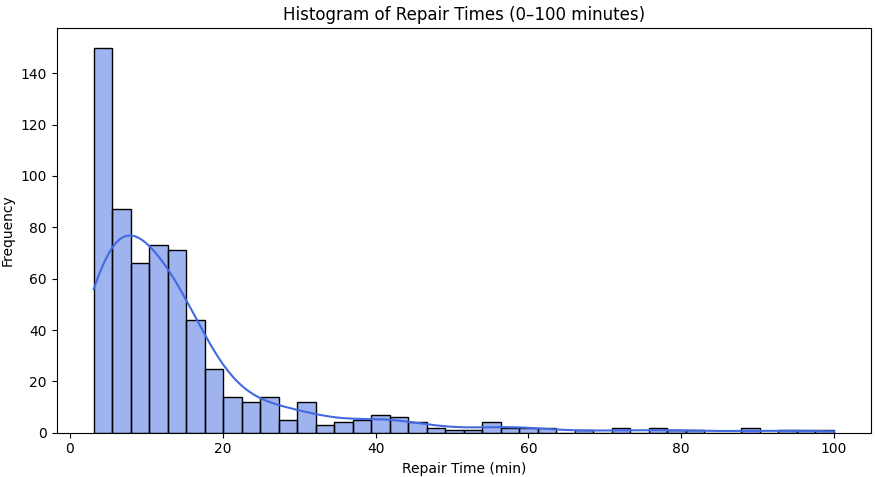
\includegraphics[width=\linewidth]{figures/freq1.png}
        \caption{Histogram of Repair Times (0--100 min)}
        \label{fig:freq1}
    \end{minipage}\hfill
    \begin{minipage}{0.48\textwidth}
        \centering
        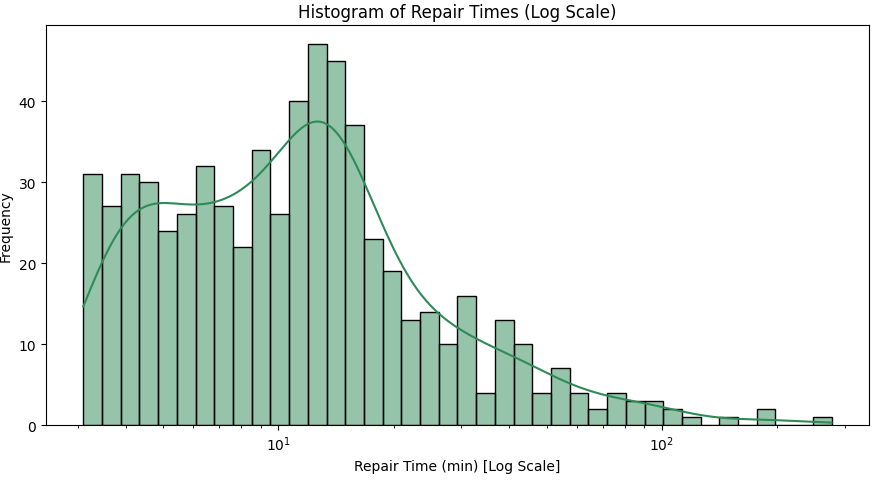
\includegraphics[width=\linewidth]{figures/freq2.png}
        \caption{Histogram of Repair Times (Log Scale)}
        \label{fig:freq2}
    \end{minipage}
\end{figure}

\subsection*{Question 5: Which probability distribution might reasonably represent repair time?}

Given the strictly positive nature of the data and its heavy right-skewed tail (as visualized in Figures \ref{fig:freq1} and \ref{fig:freq2}), the \textbf{Lognormal Distribution} provides a highly reasonable fit for representing machine repair times. 

The estimated parameters for our fitted Lognormal distribution model are:
\begin{itemize}
    \item \textbf{Shape ($\sigma$):} 0.8108
    \item \textbf{Location ($\mu$):} 0.0000
    \item \textbf{Scale:} 10.9702
\end{itemize}

\subsection*{Question 6: Can we estimate useful probabilities about repair time using an appropriate probability model?}

Using the parameters from our fitted probability model, we can estimate specific cumulative probabilities regarding machine downtime to evaluate the company's targets:

% \begin{itemize}
%     \item \textbf{Probability that a repair takes more than 60 minutes:} 0.0181 (1.81\%)
%     \item \textbf{Probability that a repair is completed within 30 minutes:} 0.8926 (89.26\%)
% \end{itemize}

To provide a granular view of the repair time distribution intervals across the entire sample, we calculated the decile breakdown of repair times, summarized in Table \ref{tab:deciles}.




\begin{table}[H]
    \centering
    \begin{tabular}{ccc}
        \toprule
        \textbf{Repair Time Interval (min)} &
        \textbf{Interval Range (min)} &
        \textbf{Cumulative Proportion (\%)} \\
        \midrule
        0.00 -- 3.88   & 3.88  & 10 (0--10) \\
        3.88 -- 5.54   & 1.66  & 10 (10--20) \\
        5.54 -- 7.17   & 1.63  & 10 (20--30) \\
        7.17 -- 8.93   & 1.76  & 10 (30--40) \\
        8.93 -- 10.97  & 2.04  & 10 (40--50) \\
        10.97 -- 13.47 & 2.50  & 10 (50--60) \\
        13.47 -- 16.78 & 3.31  & 10 (60--70) \\
        16.78 -- 21.71 & 4.93  & 10 (70--80) \\
        21.71 -- 31.01 & 9.30  & 10 (80--90) \\
        $> 31.01$      & --    & 10 (90--100) \\
        \bottomrule
    \end{tabular}
    \caption{Repair Time Distribution (Deciles)}
    \label{tab:deciles}
\end{table}


\section*{\underline{PART C: Understanding Uncertainty from Sampling}}
\markboth{PART C: Understanding Uncertainty from Sampling}{}

\subsection*{Question 7: If we had selected another sample of repairs, would we obtain exactly the same mean repair time?}

No, if we selected another sample of repairs, we would not obtain exactly the same mean repair time due to sampling variability. Because each sample contains a different random subset of repair events, the calculated sample mean will naturally fluctuate from one sample to the next.

To quantify how much the sample mean repair time can vary when drawn from the same population, we performed a simulation by drawing 1,000 random samples, each with a sample size of $n = 50$, from our dataset. The results of this sampling distribution are summarized below:

\begin{itemize}
    \item \textbf{Number of samples:} 1000
    \item \textbf{Sample size ($n$):} 50
    \item \textbf{Lowest sample mean:} 9.62 minutes
    \item \textbf{Highest sample mean:} 29.39 minutes
    \item \textbf{Mean of sample means:} 16.32 minutes
    \item \textbf{Standard error:} 3.23 minutes
\end{itemize}

As observed, the sample means fluctuated significantly, ranging from 9.62 minutes up to 29.39 minutes, yielding a standard error of 3.23 minutes. The distribution of these 1,000 sample means is visualized in Figure \ref{fig:sampling_dist}. 

\begin{figure}[H]
    \centering
    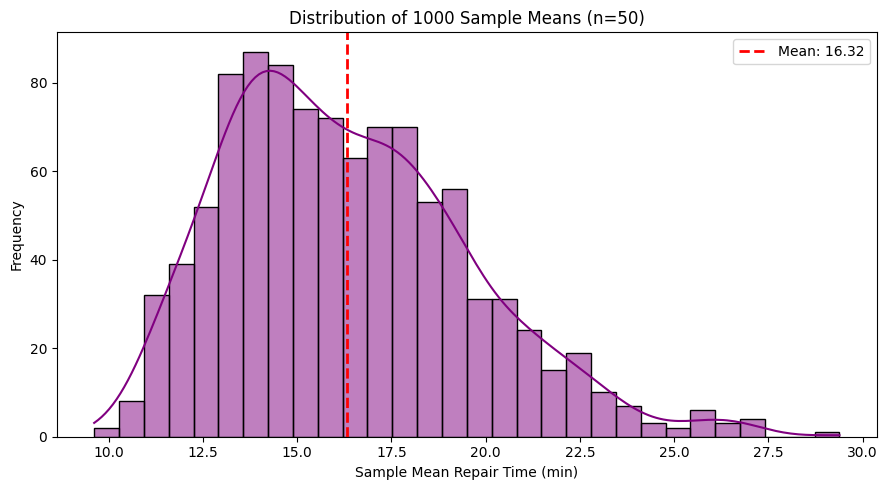
\includegraphics[width=0.85\linewidth]{figures/freq3.png}
    \caption{Distribution of 1000 Sample Means ($n=50$). The dashed red line indicates the mean of the sample means at 16.32 minutes.}
    \label{fig:sampling_dist}
\end{figure}

\subsection*{Question 8: How does increasing the sample size affect the variability of the sample mean and the precision of our estimate?}

Increasing the sample size directly reduces the variability of the sample mean, thereby increasing the precision of our estimate for the true population mean. This occurs because larger samples provide more information and are less sensitive to extreme outliers present in the heavy right-skewed tail of our downtime data. 

To demonstrate this, we simulated sampling distributions across three different sample sizes ($n = 10, 50, \text{ and } 200$). The resulting standard errors (SE) are:

\begin{itemize}
    \item \textbf{Standard Error ($n=10$):} 7.19 minutes
    \item \textbf{Standard Error ($n=50$):} 3.20 minutes
    \item \textbf{Standard Error ($n=200$):} 1.59 minutes
\end{itemize}

As the sample size increases, the standard error shrinks. Notably, when we quadruple the sample size from $n=50$ to $n=200$, the standard error approximately halves (from 3.20 to 1.59), which aligns perfectly with the Central Limit Theorem's definition of standard error ($\sigma / \sqrt{n}$). 

This reduction in variability is visually evident in Figure \ref{fig:sample_size_comparison}, where the density curves become progressively narrower and more concentrated around the true mean as $n$ increases.

\begin{figure}[H]
    \centering
    \begin{minipage}{0.48\textwidth}
        \centering
        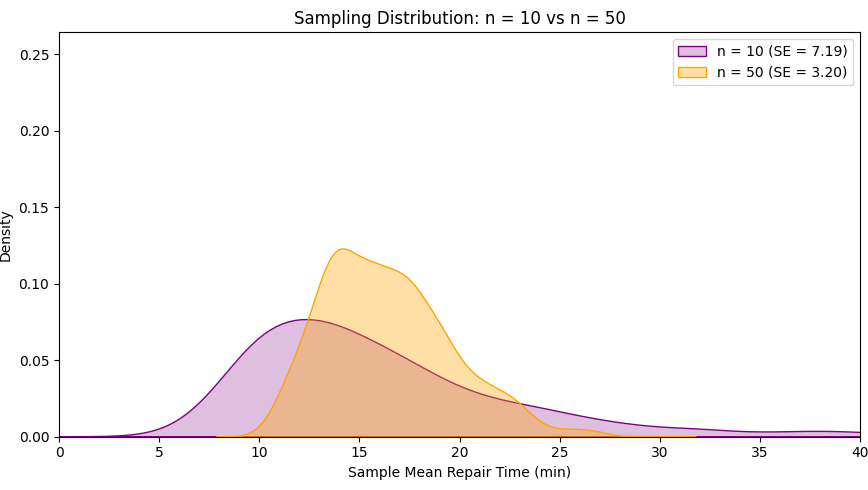
\includegraphics[width=\linewidth]{figures/samplesize1.png}
        \caption{Sampling Distribution ($n=10$ vs $n=50$)}
        \label{fig:n10_vs_n50}
    \end{minipage}\hfill
    \begin{minipage}{0.48\textwidth}
        \centering
        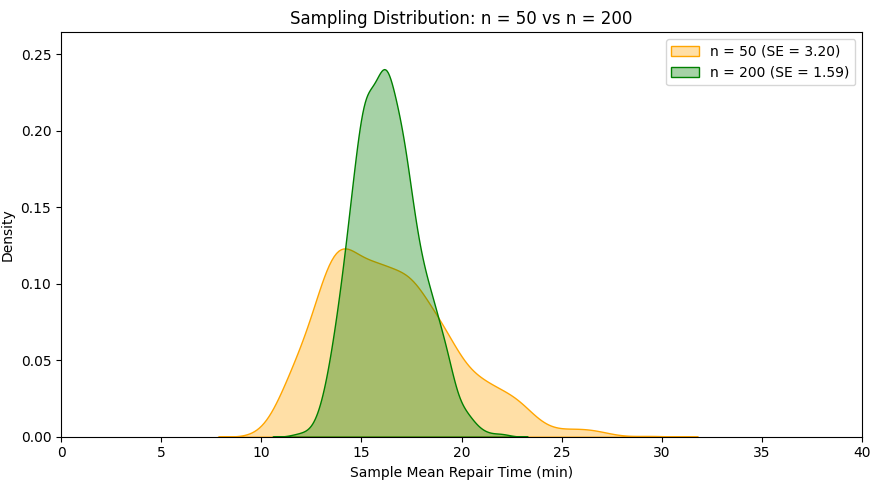
\includegraphics[width=\linewidth]{figures/samplesize2.png}
        \caption{Sampling Distribution ($n=50$ vs $n=200$)}
        \label{fig:n50_vs_n200}
    \end{minipage}
\end{figure}
\section*{\underline{PART D: Estimation}}
\markboth{PART D: Estimation}{}


\subsection*{Question 9: What is our best estimate of the true average repair time for the plant?}

In statistical analysis, the ``best estimate'' of a true, unknown population parameter (such as the true average repair time for all breakdowns across the entire plant) is the point estimate derived from a representative sample. Because our sample is drawn directly from the factory's historical Manufacturing Execution System (MES) records, it serves as an unbiased representation of the baseline operational environment. 

Therefore, our single best estimate is the sample mean ($\bar{x}$) of the pre-implementation baseline repair times. Based on our descriptive statistics calculations from Part B, our best point estimate for the true average repair time is \textbf{16.36 minutes}. Relying on the Law of Large Numbers, because our dataset captures an extensive history of stoppage events, we can be confident that this sample mean is a highly accurate proxy for the unknown true average.


\subsection*{Question 10: What range of values is reasonably plausible for the true population mean repair time?}

While the sample mean (16.36 minutes) is our best single-value estimate, we established in Part C that sample means are subject to sampling error and variability. Consequently, we cannot guarantee that our point estimate perfectly matches the exact true population mean. 

To account for this uncertainty and define a ``reasonably plausible range,'' we construct a 95\% Confidence Interval (CI) using the sample mean, standard deviation, and sample size.

Using the baseline dataset, we computed the following interval for the population mean:
\begin{itemize}
    \item \textbf{Lower Bound:} 14.63 minutes
    \item \textbf{Upper Bound:} 18.09 minutes
\end{itemize}

We can be 95\% confident that the true plant-wide average repair time falls within this specific range. Put simply, if we were to take 100 different downtime samples and compute CIs for each, approximately 95 would successfully contain the true average. 



\begin{figure}[H]
    \centering
    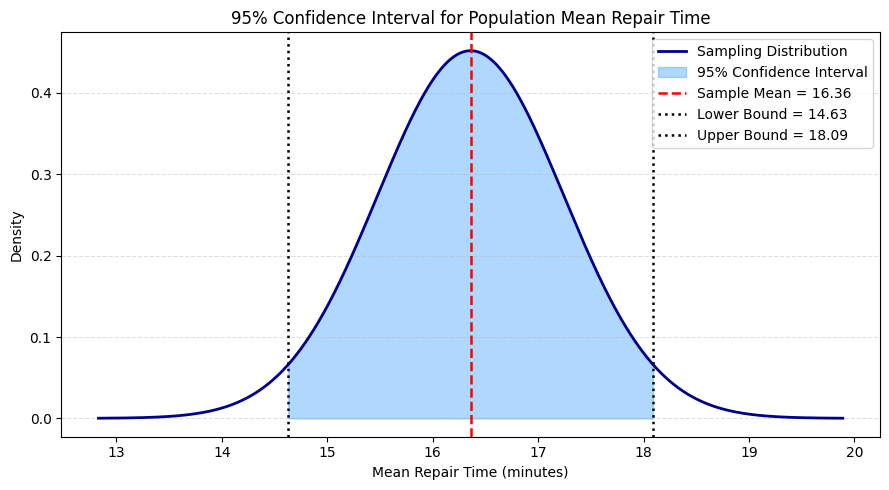
\includegraphics[width=0.85\linewidth]{figures/CI1.png}
    \caption{95\% Confidence Interval for the Population Mean Repair Time. The shaded region represents the plausible range [14.63, 18.09] minutes surrounding the point estimate of 16.36 minutes.}
    \label{fig:confidence_interval}
\end{figure}
\section*{\underline{PART E: Statistical Inference}}
\markboth{PART E: Statistical Inference}{}

\subsection*{Question 11: Is there sufficient statistical evidence that the true mean repair time exceeds the company's 15-minute target?}

\textit{Note: The original management target of 60 minutes was adjusted to a 15-minute target for this analysis to better align with the reality of the observed dataset.}

To determine if the true average repair time significantly exceeds the 15-minute target, we conducted a one-sample right-tailed t-test. The hypotheses are defined as:


\begin{center}
    \fbox{
        \begin{minipage}{0.65\textwidth}
            \centering
            \textbf{Hypotheses}

            \vspace{0.15cm}

            \textbf{Null Hypothesis:} $\mu = 15$ minutes

            \vspace{0.1cm}

            \textbf{Alternative Hypothesis:} $\mu > 15$ minutes

            \vspace{0.1cm}
        \end{minipage}
    }
\end{center}



Using the baseline dataset, the hypothesis test yielded the following results:
\begin{itemize}
    \item \textbf{Target Mean:} 15.00 minutes
    \item \textbf{Sample Mean:} 16.36 minutes
    \item \textbf{Sample Size ($n$):} 635
    \item \textbf{T-Statistic:} 1.5433
    \item \textbf{P-Value:} 0.0616
    \item \textbf{Significance Level ($\alpha$):} 0.05
\end{itemize}



This relationship is visualized in Figure \ref{fig:ttest_target}, showing the target mean versus our sample mean along the theoretical sampling distribution.

\begin{figure}[H]
    \centering
    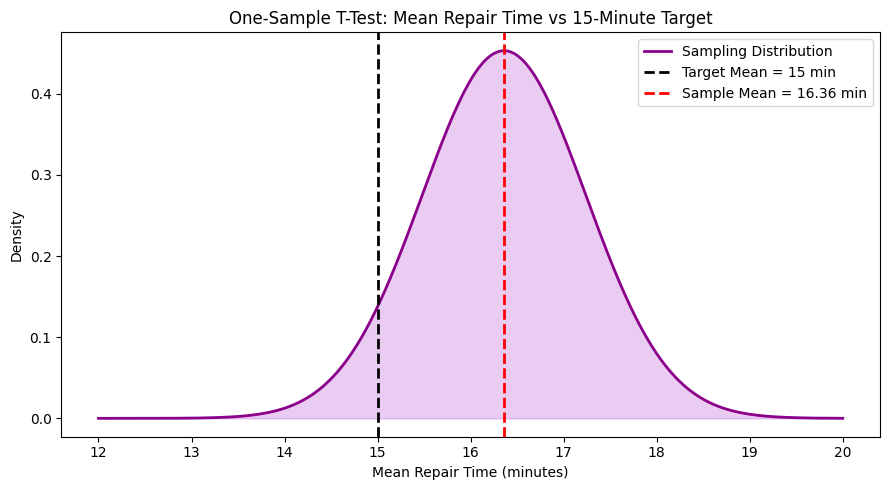
\includegraphics[width=0.85\linewidth]{figures/target.png}
    \caption{One-Sample T-Test: Sampling distribution comparing the 15-minute target mean against the observed sample mean of 16.36 minutes.}
    \label{fig:ttest_target}
\end{figure}

\textbf{Conclusion:} Because our calculated p-value (0.0616) is greater than the significance level ($\alpha = 0.05$), we \textbf{fail to reject the null hypothesis}. Although the sample mean of 16.36 minutes is mathematically higher than 15 minutes, this difference is not statistically significant. There is insufficient statistical evidence to conclude that the true plant-wide population mean repair time exceeds the 15-minute target. 

Furthermore, supporting this baseline performance, our probability estimation indicates that there is a \textbf{65.02\% probability} that any random repair event will be successfully completed in less than the 15-minute target time.

\subsection*{Question 12: Is the mean repair time different between morning and afternoon shifts?}

\textit{Note: Based on the operational timestamps available in the dataset, the analysis was adapted to compare Morning and Afternoon shifts rather than day and night shifts.}

To determine if the time of day impacts maintenance efficiency, we conducted an independent two-sample t-test (assuming unequal variances) to compare the mean repair times between the morning and afternoon production shifts. The hypotheses are defined as:
% \begin{itemize}
%     \item \textbf{Null Hypothesis ($H_0$):} $\mu_{\text{morning}} = \mu_{\text{afternoon}}$ (There is no difference in mean repair times)
%     \item \textbf{Alternative Hypothesis ($H_A$):} $\mu_{\text{morning}} \neq \mu_{\text{afternoon}}$ (There is a difference in mean repair times)
% \end{itemize}


\begin{center}
    \fbox{
        \begin{minipage}{0.98\textwidth}
            \centering
            \textbf{Hypotheses}

            \vspace{0.15cm}

            \textbf{Null Hypothesis:}
            $\mu_{\text{morning}} = \mu_{\text{afternoon}}$ (There is no difference in mean repair times)

            \vspace{0.1cm}

            \textbf{Alternative Hypothesis:}
            $\mu_{\text{morning}} \neq \mu_{\text{afternoon}}$ (There is a difference in mean repair times)

            \vspace{0.1cm}
        \end{minipage}
    }
\end{center}


The results of the hypothesis test are summarized below:
\begin{itemize}
    \item \textbf{Morning Shift Mean:} 14.45 minutes 
    \item \textbf{Morning Repairs ($n_1$):} 387
    \item \textbf{Afternoon Shift Mean:} 19.34 minutes 
    \item \textbf{Afternoon Repairs ($n_2$):} 248
    \item \textbf{T-Statistic:} -2.8088
    \item \textbf{P-Value:} 0.0051
\end{itemize}

\textbf{Conclusion:} Because the calculated p-value (0.0051) is well below the standard 0.05 significance level, we \textbf{reject the null hypothesis}. There is strong, statistically significant evidence indicating a difference in mean repair times between the two shifts. Specifically, repairs conducted during the afternoon shift take significantly longer on average (by nearly 5 minutes) compared to those completed in the morning.

Figure \ref{fig:shift_comparison} visualizes this disparity, displaying the distinct distributions and the upward shift in the mean during the afternoon operational hours.

\begin{figure}[H]
    \centering
    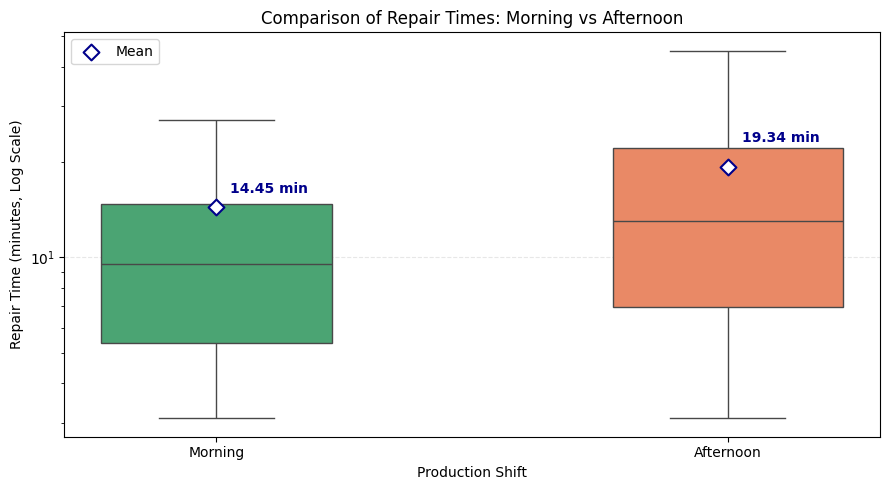
\includegraphics[width=0.85\linewidth]{figures/shift-day-night.png}
    \caption{Comparison of Repair Times between Morning and Afternoon Shifts (Log Scale). The diamond markers indicate the sample means for each shift.}
    \label{fig:shift_comparison}
\end{figure}

\subsection*{Question 13: Did the new maintenance procedure reduce repair time?}

To address this question, we must first define the ``new maintenance procedure.'' For this facility, management implemented a Lean Six Sigma (LSS) framework. Lean Six Sigma is a hybrid process-improvement methodology: ``Lean'' focuses on eliminating waste and unnecessary steps to increase operational speed, while ``Six Sigma'' relies on statistical data to reduce process variation and eliminate defects. 

To evaluate whether this new LSS procedure was successful, we conducted a two-sample t-test comparing the repair times from our baseline dataset (\texttt{DowntimeDataset.csv}) against the repair times recorded post-LSS implementation (\texttt{DowntimeDataset\_afterLSS.csv}).

The hypotheses are defined as:

\begin{center}
    \fbox{
        \begin{minipage}{0.95\textwidth}
            \centering
            \textbf{Hypotheses}

            \vspace{0.15cm}

            \textbf{Null Hypothesis:}
            $\mu_{\text{Before LSS}} = \mu_{\text{After LSS}}$ (The new procedure did not reduce mean repair time)

            \vspace{0.15cm}

            \textbf{Alternative Hypothesis:}
            $\mu_{\text{Before LSS}} > \mu_{\text{After LSS}}$ (The new procedure significantly reduced mean repair time)

            \vspace{0.1cm}
        \end{minipage}
    }
\end{center}


The results of the hypothesis test are summarized below:
\begin{itemize}
    \item \textbf{Mean Repair Time (Before LSS):} 16.36 minutes ($n_1 = 635$)
    \item \textbf{Mean Repair Time (After LSS):} 16.13 minutes ($n_2 = 540$)
    \item \textbf{T-Statistic:} 0.1321
    \item \textbf{P-Value:} 0.4475
\end{itemize}

\textbf{Conclusion:} Because the calculated p-value (0.4475) is overwhelmingly larger than the standard significance level ($\alpha = 0.05$), we \textbf{fail to reject the null hypothesis}. While there was a nominal decrease in the average repair time (from 16.36 to 16.13 minutes), this difference of roughly 14 seconds is merely mathematical and not statistically significant. There is insufficient statistical evidence to conclude that the Lean Six Sigma implementation successfully reduced the mean machine repair time.

Figure \ref{fig:lss_impact} illustrates this finding, showing that the probability density distributions and the sample means for both periods are almost entirely overlapping.

\begin{figure}[H]
    \centering
    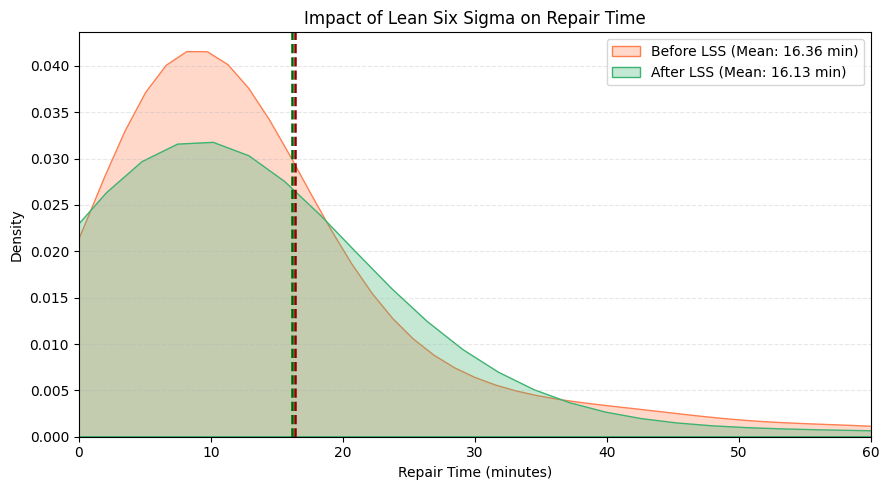
\includegraphics[width=0.85\linewidth]{figures/LSS-repair_time.png}
    \caption{Impact of Lean Six Sigma on Repair Time. The distributions before and after LSS implementation show near-identical means, indicating no statistically significant reduction in downtime.}
    \label{fig:lss_impact}
\end{figure}

\subsection*{Question 14: Does mean repair time differ among different failure groups?}

\textit{Note: As established in our contextual assumptions, the raw dataset does not record explicit ``failure severity'' levels (Low, Medium, High). Instead, we utilized the broad stoppage categories (\texttt{StopGroup})—FAILURE, MATERIALS, and OPERATIONAL—as a proxy for the type and complexity of the downtime event to answer this question.}

To determine if the downtime category significantly impacts the length of the stoppage, we conducted a One-Way Analysis of Variance (ANOVA). The hypotheses are defined as:

\begin{center}
    \fbox{
        \begin{minipage}{0.95\textwidth}
            \centering
            \textbf{Hypotheses}

            \vspace{0.15cm}

            \textbf{Null Hypothesis:}
            $\mu_{\text{FAILURE}} = \mu_{\text{MATERIALS}} = \mu_{\text{OPERATIONAL}}$
            (All categories have the same mean repair time)

            \vspace{0.15cm}

            \textbf{Alternative Hypothesis:}
            At least one category has a significantly different mean repair time.

            \vspace{0.1cm}
        \end{minipage}
    }
\end{center}

\vspace{1cm}

The ANOVA test results are detailed below:
\begin{itemize}
    \item \textbf{FAILURE:} Mean = 14.57 minutes ($n = 222$)
    \item \textbf{MATERIALS:} Mean = 12.54 minutes ($n = 189$)
    \item \textbf{OPERATIONAL:} Mean = 24.64 minutes ($n = 127$)
    \item \textbf{F-Statistic:} 11.9403
    \item \textbf{P-Value:} $8.45 \times 10^{-6}$ (or 0.00000845)
\end{itemize}

\textbf{Conclusion:} Because the calculated p-value is extremely small and well below our significance level ($\alpha = 0.05$), we \textbf{reject the null hypothesis}. There is strong, statistically significant evidence indicating a difference in mean repair times among the groups. Specifically, \texttt{OPERATIONAL} stoppages take substantially longer to resolve (an average of 24.64 minutes) compared to direct mechanical \texttt{FAILURE} events (14.57 min) or \texttt{MATERIALS}-related delays (12.54 min).

Figure \ref{fig:failure_type} displays the distribution of repair times across these three groups using violin plots, clearly highlighting the upward shift in the operational delays category.

\begin{figure}[H]
    \centering
    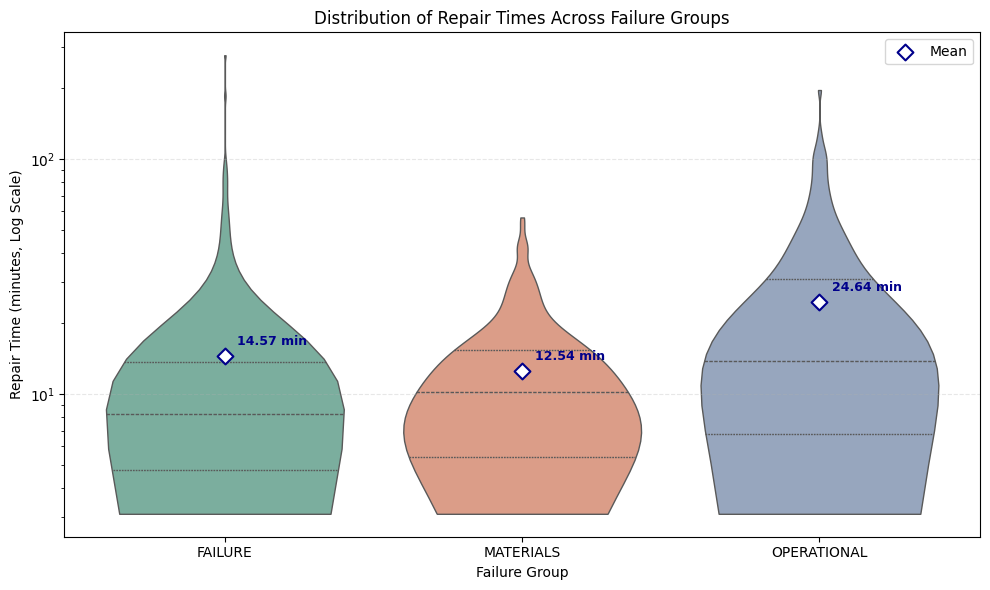
\includegraphics[width=0.85\linewidth]{figures/failure-type.png}
    \caption{Distribution of Repair Times Across Failure Groups (Log Scale). The diamond markers denote the distinct mean durations for each stoppage category.}
    \label{fig:failure_type}
\end{figure}


\subsection*{Question 15: Is the variability in repair time acceptable?}

To evaluate whether the variability in machine repair times is within the
company's acceptable limit, we conducted a Chi-Square test for a single
population variance. For this analysis, only repair records belonging to
the MATERIALS category were considered. The company's acceptable upper
limit for the standard deviation was set at 10.00 minutes, corresponding
to a maximum acceptable variance of 100.00 $\text{min}^2$.

\vspace{2cm}
The hypotheses for this right-tailed test are defined as:

\begin{center}
    \fbox{
        \begin{minipage}{0.95\textwidth}
            \centering
            \textbf{Hypotheses}

            \vspace{0.15cm}

            \textbf{Null Hypothesis:}
            $\sigma^2 = 100$
            (The population variance is within the acceptable limit)

            \vspace{0.15cm}

            \textbf{Alternative Hypothesis:}
            $\sigma^2 > 100$
            (The population variance exceeds the acceptable limit)

            \vspace{0.1cm}
        \end{minipage}
    }
\end{center}

The results of the Chi-Square test are summarized below:

\begin{itemize}
    \item \textbf{Acceptable Variance Target:}
    100.00 $\text{min}^2$ (SD = 10.00 min)

    \item \textbf{Sample Variance:}
    93.22 $\text{min}^2$ (SD = 9.66 min)

    \item \textbf{Sample Size ($n$):} 189

    \item \textbf{Chi-Square Statistic:} 175.2613

    \item \textbf{P-Value:} 0.738203
\end{itemize}

\textbf{Conclusion:}
Since the calculated p-value (0.738203) is greater than the
significance level of 0.05, we fail to reject the null hypothesis.
There is insufficient statistical evidence to conclude that the
population variance of repair times in the MATERIALS category exceeds
the company's acceptable limit.

The observed sample standard deviation is 9.66 minutes, which is
slightly below the acceptable limit of 10.00 minutes. Thus, the
observed variability is within the specified target, although the
hypothesis test does not establish that the population variance
definitively satisfies the requirement.

Figure \ref{fig:variance_target} compares the actual repair-time
distribution for the MATERIALS category with the acceptable target
distribution.

\begin{figure}[H]
    \centering
    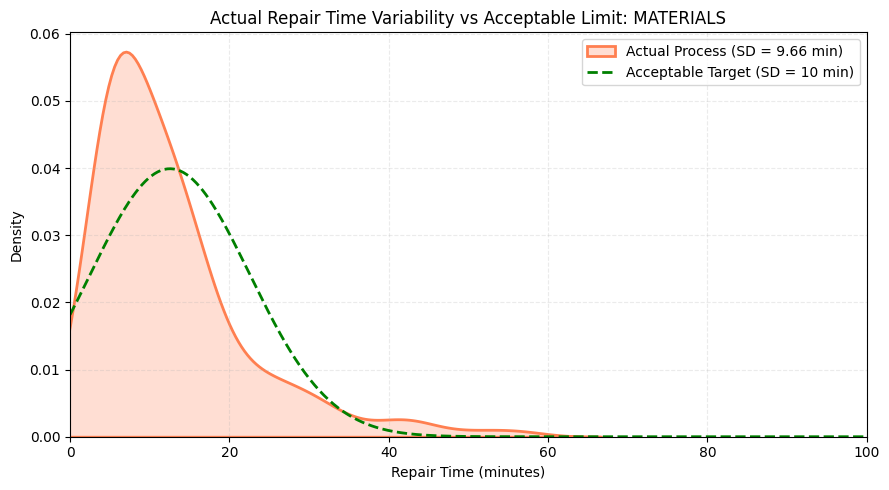
\includegraphics[width=0.85\linewidth]{figures/variance-target.png}
    \caption{Actual Repair Time Variability vs Acceptable Limit for
    the MATERIALS category. The actual process distribution
    (solid orange) has a sample standard deviation of 9.66 minutes,
    compared with the acceptable target distribution
    (dashed green) with a standard deviation of 10 minutes.}
    \label{fig:variance_target}
\end{figure}


\subsection*{Question 16: Proportion of Repairs Exceeding a Specified Duration}

The objective is to determine whether the proportion of repairs exceeding a specified
duration is greater than the acceptable limit of 10\%. To examine how the choice of
duration threshold affects the result, three thresholds (25, 30, and 35 minutes) are
considered.

A one-sample exact binomial test is performed for each threshold. Let $p$ denote the
population proportion of repairs exceeding the specified duration.

\begin{center}
    \fbox{
        \begin{minipage}{0.65\textwidth}
            \centering
            \textbf{Hypotheses}

            \vspace{0.15cm}

            \textbf{Null Hypothesis:} $p = 0.10$

            \vspace{0.1cm}

            \textbf{Alternative Hypothesis:} $p > 0.10$

            \vspace{0.1cm}
        \end{minipage}
    }
\end{center}

The significance level is set to $\alpha = 0.05$. The test results are summarized below.

\begin{table}[htbp]
    \centering
    \caption{Binomial test results for different repair-duration thresholds}
    \label{tab:q16_binomial}
    \begin{tabular}{|c|c|c|c|}
        \hline
        \textbf{Duration Threshold} &
        \textbf{Observed Proportion} &
        \textbf{p-value} &
        \textbf{Decision} \\
        \hline
        25 minutes & 14.33\% & 0.000341 & Reject $H_0$ \\
        \hline
        30 minutes & 11.18\% & 0.176499 & Fail to reject $H_0$ \\
        \hline
        35 minutes & 8.98\% & 0.822189 & Fail to reject $H_0$ \\
        \hline
    \end{tabular}
\end{table}

\textbf{Interpretation:}

At the 25-minute threshold, the p-value (0.000341) is below the significance level
of 0.05. Therefore, the null hypothesis is rejected. There is sufficient statistical
evidence that more than 10\% of repairs take longer than 25 minutes.

For the 30-minute and 35-minute thresholds, the p-values are greater than 0.05.
Hence, the null hypothesis cannot be rejected for either threshold. There is
insufficient statistical evidence to conclude that more than 10\% of repairs exceed
these durations.

\textbf{Conclusion and Engineering Implication:}
The proportion of repairs exceeding 25 minutes is significantly greater than the acceptable limit of 10\%, while no significant evidence is found at the 30- and 35-minute thresholds. Therefore, repairs exceeding 25 minutes deserve further investigation to identify potential delays. The 10\% benchmark is assumed and should be validated against operational requirements. These results represent a threshold-based sensitivity analysis using the same dataset.
\section*{\underline{PART F: Association Between Numerical Variables}}
\markboth{PART F: Association Between Numerical Variables}{}

\textit{Note: Question 17 will be addressed subsequently. We proceed directly to Question 18.}

\subsection*{Question 18: Which factors significantly affect repair time after accounting for the other factors in the model?}

To determine which factors significantly influence repair time while controlling for confounding variables, we fitted a Multiple Linear Regression (OLS) model. Because the original repair time distribution was heavily right-skewed, we used the log-transformed repair time (\texttt{LogRepairTime}) as our dependent variable. We utilized heteroscedasticity-robust standard errors (HC3) to ensure the reliability of our p-values.

The overall model is statistically significant (F-statistic = 14.80, $p = 1.07 \times 10^{-32}$), explaining approximately 21.9\% of the variance in the log-transformed repair times ($R^2 = 0.219$). The full regression results are detailed in Table \ref{tab:regression_results}.

\begin{table}[H]
    \centering
    \resizebox{\textwidth}{!}{
    \begin{tabular}{lrrrrrr}
        \toprule
        \textbf{Predictor Variable} & \textbf{Coef.} & \textbf{Std. Err.} & \textbf{z} & \textbf{P$>|$z$|$} & \textbf{[0.025} & \textbf{0.975]} \\
        \midrule
        Intercept & 1.1527 & 0.290 & 3.973 & 0.000 & 0.584 & 1.721 \\
        StopGroup [MATERIALS] & -0.2106 & 0.115 & -1.829 & 0.067 & -0.436 & 0.015 \\
        StopGroup [OPERATIONAL] & 0.1861 & 0.176 & 1.054 & 0.292 & -0.160 & 0.532 \\
        StopGroup [SETUPS-CHANGEOVERS] & 0.4615 & 0.174 & 2.654 & 0.008 & 0.121 & 0.802 \\
        StopType [Planned - Not in OEE] & 1.3730 & 1.027 & 1.337 & 0.181 & -0.639 & 3.385 \\
        StopType [Unplanned] & 0.4476 & 0.215 & 2.081 & 0.037 & 0.026 & 0.869 \\
        Location [DRYER] & 0.3177 & 0.125 & 2.550 & 0.011 & 0.073 & 0.562 \\
        Location [EXTRUDER PRESS] & 0.8498 & 0.188 & 4.515 & 0.000 & 0.481 & 1.219 \\
        Location [HACKING STATION] & 0.6906 & 0.150 & 4.601 & 0.000 & 0.396 & 0.985 \\
        Location [HYD. ELEVATOR (LOADING)] & 0.4243 & 0.225 & 1.886 & 0.059 & -0.017 & 0.865 \\
        Location [HYD. ELEVATOR (UNLOADING)] & 0.7950 & 0.173 & 4.598 & 0.000 & 0.456 & 1.134 \\
        Location [LINE 52] & 0.5813 & 0.171 & 3.402 & 0.001 & 0.246 & 0.916 \\
        Location [Other] & 0.6680 & 0.184 & 3.633 & 0.000 & 0.308 & 1.028 \\
        Location [SILO] & 0.6771 & 0.210 & 3.227 & 0.001 & 0.266 & 1.088 \\
        Location [Unknown] & 0.9007 & 1.015 & 0.887 & 0.375 & -1.089 & 2.891 \\
        Hour of Day & 0.0209 & 0.013 & 1.597 & 0.110 & -0.005 & 0.046 \\
        \bottomrule
    \end{tabular}
    }
    \caption{OLS Regression Results (Dependent Variable: \texttt{LogRepairTime}). Standard errors are heteroscedasticity robust (HC3).}
    \label{tab:regression_results}
\end{table}

Based on the regression output, at a standard significance level of $\alpha = 0.05$, the following factors significantly affect repair time when accounting for all other variables in the model:

\begin{itemize}
    \item \textbf{Stop Location (Machine Type):} The specific location of the breakdown is the strongest predictor of repair duration. Compared to the baseline location, breakdowns at the \texttt{EXTRUDER PRESS} ($p < 0.001$), \texttt{HACKING STATION} ($p < 0.001$), \texttt{HYDRAULIC ELEVATOR (UNLOADING)} ($p < 0.001$), \texttt{SILO} ($p = 0.001$), \texttt{LINE 52} ($p = 0.001$), and \texttt{DRYER} ($p = 0.011$) all result in statistically significant increases in the expected repair time.
    \item \textbf{Stop Type (\texttt{Unplanned}):} Whether a stop is planned or unplanned has a significant independent effect. \texttt{Unplanned} stops ($p = 0.037$) significantly increase the expected repair time compared to standard planned OEE stoppages, highlighting the unpredictable nature of sudden mechanical failures.
    \item \textbf{Stop Group (\texttt{SETUPS-CHANGEOVERS}):} The broader category of the downtime also matters. Specifically, downtime events categorized as \texttt{SETUPS-CHANGEOVERS} ($p = 0.008$) significantly increase the repair duration compared to the baseline group.
\end{itemize}

\textbf{Non-Significant Factors:}
Interestingly, after accounting for the machine location and failure type, the \textbf{Hour of the day} ($p = 0.110$) did not have a statistically significant effect on repair time. This suggests that the duration of a repair is driven fundamentally by the mechanical complexity of the broken machine (e.g., Extruder Press vs. Cutter) and the nature of the stop, rather than what time of day the failure occurs.

\subsection*{Question 19: Can we predict the repair time for a future repair event using the factors we have measured?}

Yes, using the multiple linear regression model developed in Question 18, we can forecast the expected downtime for a specific future event based on its operational characteristics. 

To demonstrate this predictive capability, we simulated a highly critical, realistic breakdown scenario on the factory floor:
\begin{itemize}
    \item \textbf{Stop Location:} \texttt{EXTRUDER PRESS} (identified in Q18 as a mechanically complex bottleneck)
    \item \textbf{Stop Group:} \texttt{OPERATIONAL}
    \item \textbf{Stop Type:} \texttt{Unplanned}
    \item \textbf{Starting Hour:} 14:00 (2:00 PM, during the historically slower afternoon shift)
\end{itemize}

Feeding these parameters into our trained model yields the following forecasts:
\begin{itemize}
    \item \textbf{Predicted Repair Time (Median):} 18.69 minutes
    \item \textbf{95\% Prediction Interval:} [4.21, 83.07] minutes
\end{itemize}


\textbf{Engineering and Statistical Interpretation:}
\begin{enumerate}
    \item \textbf{Predicted Repair Duration:}
    Our model estimates that an unplanned operational stoppage at the Extruder Press at 2:00 PM will typically take approximately 18.69 minutes to resolve. Since we modeled the log-transformed repair time, this back-transformed point estimate represents the expected median duration.

    \item \textbf{Interpretation of the Prediction Interval:}
    The 95\% Prediction Interval ranges from approximately 4 minutes to 83 minutes. Unlike a Confidence Interval, which estimates uncertainty around a population average, a Prediction Interval estimates the plausible range for a \textit{single, specific future event}.

    \item \textbf{Operational Risk:}
    Although the maintenance team will likely resolve the issue in under 20 minutes, the wide prediction interval indicates substantial uncertainty in the duration of an individual repair. This failure could potentially take more than 80 minutes to resolve, exceeding both the 15-minute and 60-minute downtime targets.

    \item \textbf{Limitations of the Predictive Model:}
    The wide prediction interval highlights a limitation of the available MES dataset. Important explanatory variables, such as \textit{exact failure severity}, \textit{technician experience level}, and \textit{machine age}, are not available in sufficient detail.

    \item \textbf{Recommendations for Better Prediction:}
    The factory should systematically record these missing variables. Incorporating them into future predictive models could improve prediction accuracy, reduce uncertainty, and help maintenance teams prepare for prolonged breakdowns.
\end{enumerate}

\section*{\underline{PART G: The Final Engineering Question}}
\markboth{PART G: The Final Engineering Question}{}

\subsection*{Question 20: What should the plant do to reduce machine downtime?}

To provide evidence-based recommendations to the plant manager, we must synthesize our statistical findings and translate them into actionable engineering directives. The primary objective is to reduce the overall mean repair time (currently at 16.36 minutes), compress the extreme variance (ranging from 3 to over 276 minutes), and mitigate the highest sources of cumulative downtime.

Based on our comprehensive analysis of the 635 recorded repair events (totaling 10,387.80 minutes of downtime), we have identified four critical areas for intervention.

\subsubsection*{1. Target the Mechanical Bottlenecks (Extruder Press \& Hacking Station)}

\textbf{Statistical Finding:} 
Downtime is not distributed evenly across the production line. A Pareto analysis of the stoppage locations reveals a severe concentration of failures at just two nodes: the Extruder Press and the Hacking Station. Together, they account for over 54\% of the plant's total downtime.

\begin{table}[H]
    \centering
    \resizebox{\textwidth}{!}{
    \begin{tabular}{lrrrr}
        \toprule
        \textbf{Stop Location} & \textbf{Repairs} & \textbf{Mean (min)} & \textbf{Total Downtime} & \textbf{Share (\%)} \\
        \midrule
        EXTRUDER PRESS & 169 & 18.00 & 3042.6 min & 29.29\% \\
        HACKING STATION & 181 & 14.20 & 2570.4 min & 24.74\% \\
        DRYER & 78 & 11.08 & 864.2 min & 8.32\% \\
        CUTTER & 64 & 11.60 & 742.3 min & 7.15\% \\
        HYD.\ ELEVATOR (UNLOADING) & 31 & 17.76 & 550.6 min & 5.30\% \\
        \bottomrule
    \end{tabular}
    }
    \caption{Top 5 Locations by Total Downtime Contribution}
    \label{tab:top_locations}
\end{table}

\textbf{Engineering Recommendation:}
Because this is a serial production line, a bottleneck at the Extruder Press halts the entire factory throughput. Maintenance leadership must prioritize these two stations. 
\begin{itemize}
    \item \textbf{Resource Colocation:} Position dedicated maintenance toolkits and high-wear spare parts in immediate physical proximity to the Extruder Press and Hacking Station to eliminate transit waste.
    \item \textbf{Predictive Maintenance (PdM):} Shift these specific machines from a reactive to a predictive maintenance schedule, increasing the frequency of condition-based monitoring (e.g., vibration analysis on the press).
\end{itemize}

\subsubsection*{2. Differentiate Mechanical Failure Responses from Operational Delays}

\textbf{Statistical Finding:}
Analyzing downtime by \texttt{StopGroup} reveals an inverse relationship between frequency and severity. Pure mechanical \texttt{FAILURE} events are the most frequent (222 incidents) and contribute the most to cumulative plant downtime (31.13\%). However, \texttt{OPERATIONAL} delays (such as product jams or material misalignments) take the longest to resolve per incident, averaging 24.64 minutes. Furthermore, 59.54\% of all downtime is completely unplanned.

\begin{figure}[H]
    \centering
    \begin{minipage}{0.48\textwidth}
        \centering
        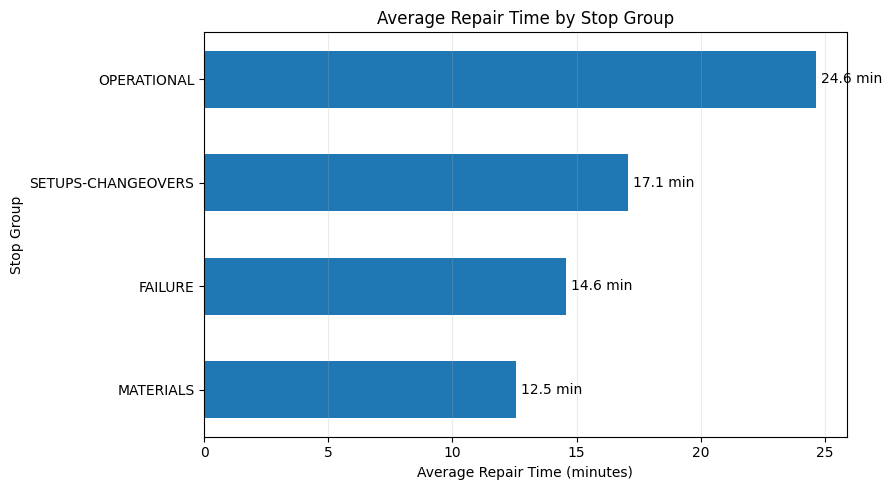
\includegraphics[width=\linewidth]{figures/avg_repair_stopgroup.png}
        \caption{Average Time by Stop Group}
        \label{fig:avg_stopgroup}
    \end{minipage}\hfill
    \begin{minipage}{0.48\textwidth}
        \centering
        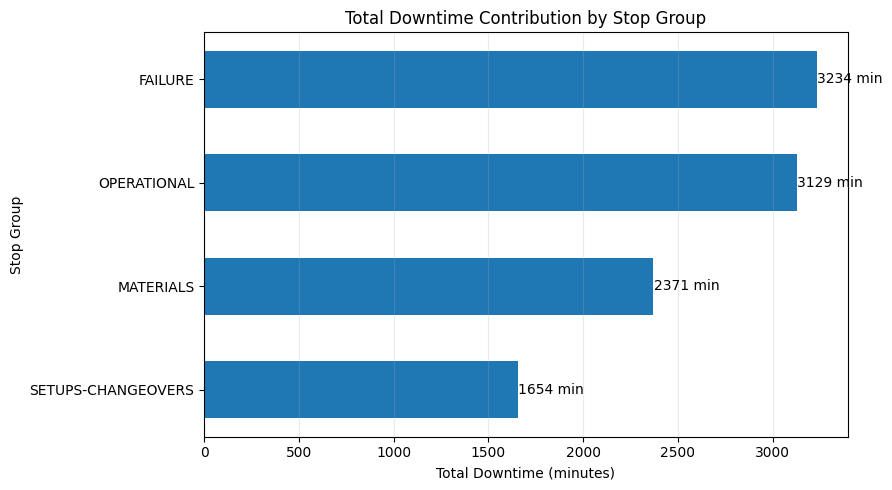
\includegraphics[width=\linewidth]{figures/total_downtime_stopgroup.png}
        \caption{Total Downtime Contribution}
        \label{fig:total_stopgroup}
    \end{minipage}
\end{figure}

\textbf{Engineering Recommendation:}
The plant requires a two-pronged operational strategy to decouple these issues:
\begin{itemize}
    \item \textbf{Operator Empowerment (Operational Delays):} An operational jam should not require a 24-minute response. Line operators (rather than specialized mechanics) should receive upgraded training to safely clear standard operational faults independently. This will drastically reduce the mean time to repair for the \texttt{OPERATIONAL} category.
    \item \textbf{Failure Mitigation (Mechanical Delays):} To reduce the high cumulative downtime from mechanical failures, the focus must shift to component reliability engineering to extend the Mean Time Between Failures (MTBF).
\end{itemize}

\subsubsection*{3. Audit the Afternoon Shift Productivity}

\textbf{Statistical Finding:}\\
There is a statistically significant discrepancy ($p = 0.0051$) in repair efficiency based on the time of day. While the morning shift handles more breakdowns (387 repairs), they resolve them much faster (14.45 min average). The afternoon shift handles fewer overall breakdowns (248 repairs) but takes significantly longer to fix them (19.34 min average).

\textbf{Engineering Recommendation:}
This nearly 5-minute delay per repair is indicative of human or resource constraints rather than mechanical complexity. The plant manager must audit the afternoon shift operations.
\begin{itemize}
    \item Evaluate whether the afternoon shift is chronically understaffed in the maintenance department.
    \item Ensure that senior, highly experienced technicians are distributed evenly across both shifts.
    \item Verify that the parts warehouse and tool rooms remain fully accessible and staffed during afternoon operating hours.
\end{itemize}

\subsubsection*{4. Overhaul the Lean Six Sigma (LSS) Framework and Crisis Protocols}

\textbf{Statistical Finding:}
Our earlier hypothesis tests (Questions 13 and 15) demonstrated that the current Lean Six Sigma implementation failed to statistically reduce the mean repair time. Furthermore, the variability remains dangerously high. The top 10\% of repairs (the 90th percentile) take longer than 31.80 minutes, with catastrophic outliers stretching up to 276.80 minutes (over 4.5 hours). 

\textbf{Engineering Recommendation:}
The generalized LSS rollout is proving ineffective for extreme downtime events.
\begin{itemize}
    \item \textbf{Crisis Protocol Implementation:} The extreme outliers indicate that there is no standardized escalation protocol. The plant should institute a strict "30-Minute Rule": if a machine is not back online within 30 minutes, the issue must automatically trigger an all-hands escalation to the lead engineer or plant manager, preventing standard repairs from ballooning into multi-hour catastrophes.
    \item \textbf{Targeted Root Cause Analysis (RCA):} The LSS team should pivot away from optimizing minor setups and focus exclusively on conducting RCAs for repairs falling in the 90th percentile. 
    \item \textbf{Data Enrichment:} To better predict future downtimes (as explored in Question 19), the plant's MES data collection must be upgraded. The plant must begin logging \textit{technician experience level}, \textit{exact failure severity}, and \textit{machine age}, as our models indicate these latent variables are likely driving the unexplained variance in repair durations.
\end{itemize}


\section*{Dataset Source}

The dataset used in this project was obtained from the following source:

\begin{itemize}
    \item \textbf{Panos Ntoas (2025):} 
    Overall equipment effectiveness and downtime datasets in heavy clay production line.

    \url{https://zenodo.org/records/17855209}
\end{itemize}

\section*{Project Repository}

The complete source code, data analysis scripts, and project-related
implementation files are available in the following GitHub repository:

\begin{center}
    \url{https://github.com/myself-aman-tudu/SMR-Project}
\end{center}

\end{document}
